%!TEX root = ../template.tex
%%%%%%%%%%%%%%%%%%%%%%%%%%%%%%%%%%%%%%%%%%%%%%%%%%%%%%%%%%%%%%%%%%%%
%% chapter3.tex
%% NOVA thesis document file
%%
%% Chapter with a short latex tutorial and examples
%%%%%%%%%%%%%%%%%%%%%%%%%%%%%%%%%%%%%%%%%%%%%%%%%%%%%%%%%%%%%%%%%%%%

\typeout{NT FILE chapter3.tex}%

\makeatletter
\newcommand{\ntifpkgloaded}{%
  \@ifpackageloaded%
}
\makeatother


\chapter{System Model \& Software Architecture}\label{cha:system_model}

This chapter provides an in-depth analysis of the system model and software architecture of Packet Padding Cells and Jitter Induction Schedulers features. 
We begin by introducing the system's overall and foundational principles. 
Next, we present detailed breakdown of the system model architecture. 
Subsequently, we present the threat model, analyzing the potential threats and adversaries accounted for both features' design. 
Then, we explain the software architecture of the solution, compared with the Tor's architecture.
Finally, we conclude with a comprehensive summary that synthesizes the key insights discussed throughout the chapter.

\section{Packet Padding Cells and Jitter Induction Schedulers Proposal}\label{sec:system_propostal}

As discussed previously in \autoref{sec:motivation}, Tor is a widely used anonymity network that provides users privacy and anonymity while browsing the internet. However, advances in machine learning and data analysis have made it possible to de-anonymize Tor users by analyzing their traffic patterns, therefore potentially  compromising the privacy and anonymity that Tor aims to provide~\cite{chakravarty2014trafficanalysis, johnson2013users,winter2012great,robjansen2019dosontor}. 

This can be achieved through some traffic analysis attacks, such as fingerprinting and traffic correlation. As discussed in \autoref{sec:problem}, these traffic analysis attacks represent a significant threat to Tor users' privacy and anonymity, as sophisticated adversaries can use the above-mentioned techniques to analyze monitored traffic patterns and de-anonymize users and their browsing activities.

Therefore, we propose Packet Padding Cells (PPC) and Jitter Induction Schedulers (JIS), an extension of Tor source code that includes a Differential Privacy TLS packet padding mechanism based on false Tor cells generation and two jitter injection Tor schedulers with various mathematical distributions to protect the users' data and prevent de-anonymization attacks. By incorporating Differential Privacy and injecting variable and randomized jitter into the Tor traffic, we have obfuscated its patterns and increased the network's resistance against fingerprinting and correlation attacks.

The main goal of both PPC and JIS is to reinforce Tor's resistance against traffic analysis attacks, especially fingerprinting and correlation, thus fortifying users' privacy and anonymity, and ensuring that the solution maintains reasonable performance and usability. To achieve this goal, we designed both features with the following goals in mind:
\paragraph{Formally Proven:} The solution must be formally proven to provide a certain level of privacy, by using Differential Privacy. This way, we add a new and important layer of security and trust to the Tor network and users.
\paragraph{Tor's Extension:} The solution must be an extension of the Tor project, respecting Tor's design principles and rules. As a very popular open source project, Tor has a large community of users and developers, and it is important to ensure that the solution can be easily integrated into the existing Tor source code.
\paragraph{Compatibility:} The Tor network is composed of numerous voluntary relays operated by independent hosts. Therefore, the proposed solution must be easily integrated into the existing Tor infrastructure and remain compatible with relays that are unaware of it.
\paragraph{Unobservability:} The solution must enhance Tor's resistance against traffic analysis attacks, specifically fingerprinting and correlation attacks, in comparison to the existing Tor network. 
\paragraph{Configurability:} As an extension of the Tor project, the solution must use the existing Tor configuration files and allow users and hosts to configure the trade-offs between privacy and performance, where users can choose the level of privacy they want to achieve.
\paragraph{Performance:} We consider that performance is a key aspect of the solution. Even though the solution does not aim to improve the performance of the Tor network, to allow this solution to be relevant and useful for the Tor software and community, it is important to ensure that the solution does not significantly impact the performance of the Tor network negatively. 


\section{System Model}\label{sec:system_model}

As stated previously, the solution is an extension of the Tor project, so the system model is also similar to the Tor's system model, as briefly explained in Section~\ref{sec:tor_network}. In order to preserve the Tor network's design principles and rules, our system model does not introduce any new components or mechanisms in the network layer of the system, as illustrated in~\autoref{fig:system_model}. 

\begin{figure}[!h]
  \centering
  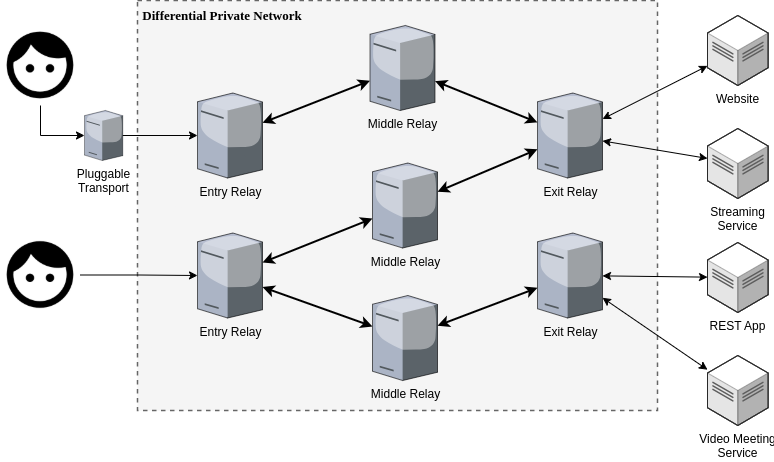
\includegraphics[width=\textwidth]{Chapters/Figures/System_Model_Geral.png}
  \caption{Differential Private Network System Model}\label{fig:system_model}
\end{figure}

Instead, it focuses on enhancing the scheduling on existing Tor relays, with the proposed Jitter Injection Schedulers, and on introducing a new mechanism for generating additional traffic, called \textit{Packet Padding Cells} mechanism, which are both presented further below.

\paragraph{Jitter Injection Schedulers (JIS):} A pair of schedulers for Tor cells that incorporates mathematical distributions techniques to apply random jitter conditions to the Tor network traffic. By setting a random interval between scheduler runs, we are able to apply jitter to the Tor network traffic, making it more difficult for adversaries to analyze the traffic patterns and de-anonymize users. As each scheduler can or not apply a delay, the jitter is applied by each individual relay and/or client, making the privacy properties accumulate across the network, therefore providing a stronger privacy guarantee further the cell lives and travels through the network.
\paragraph{Packet Padding Cells (PPC):} A mechanism that generates additional traffic by creating false Tor cells to the network traffic. These cells are generated based on a decision-making differential private mechanism triggered when the relay receives a new Tor \texttt{relay} cell. The newly generated cells are added to the circuit cell queue of the original cell, which leads to the generated traffic to only be added to active and established circuits.  In comparison to the above schedulers, the privacy properties do not accumulate across the network, as the cells are generated only when a new Tor cell is received, and discarded on reception. 
In this case, 2 adjacent segments will have the same amount of Packet Padding Cells, but the ones created by the initial relay will be discarded by the second and the last relay will only receive the false cells generated by the second relay, also meaning that the TLS packet count won't be coupled to the number of cells created nor to a certain pattern shared by all segments. Additionally, the client does not produce any additional traffic, unlike the Schedulers.

These two new features are designed to work independently, meaning that the user can choose to use one or both of them, but with the same goal of enhancing the Tor network's resistance against traffic analysis attacks.


\section{Threat Model}\label{sec:threat_model}

As mentioned earlier, Tor network is widely used anonymity network that may be vulnerable to traffic analysis attacks, such as fingerprinting and traffic correlation. Considering these types of attacks, adversaries analyze and monitor traffic in certain segments of the network, aiming to gather information to train and strengthen their machine and deep learning models, which can then be used to de-anonymize users and expose their browsing activities, for example. This way, users that browse the internet through the Tor network may be vulnerable to these attacks, which can lead to the exposure of their browsing activities and identities, and making Tor inefficient. 

The proposed solution is designed to strengthen the Tor network's privacy guarantees and bolster its defenses against traffic analysis attacks, with a particular focus on the before mentioned threats. While developing our threat model, we closely follow the foundational Tor threat model outlined by \autocite{dingledine2004tor}~\cite{dingledine2004tor}, taking into consideration adversaries whose ultimate objective is the de-anonymization of users and the exposure of their browsing activities, and which are able to monitor portions of network traffic, manipulate data flows, and compromise a fraction of existing routers.

Before defining our adversary model, we first clarify the types of adversaries considered and which are not included in our threat model. State-Level adversaries (SLAd) are capable of observing Tor's traffic patterns in one or few Autonomous Systems (AS). Large-Scope adversaries (LSAd) are considered a group of SLAd that can monitor a significant fraction of the network, by collaborating and working together and therefore controlling the collection of regions controlled by each collaborator. Finally, Omnipresent adversaries (OPAd) are a powerful attacker, or a group of attackers, that can monitor the entire Tor network, including all segments and regions, and therefore can observe all traffic patterns.

\begin{figure}[!h]
  \centering
  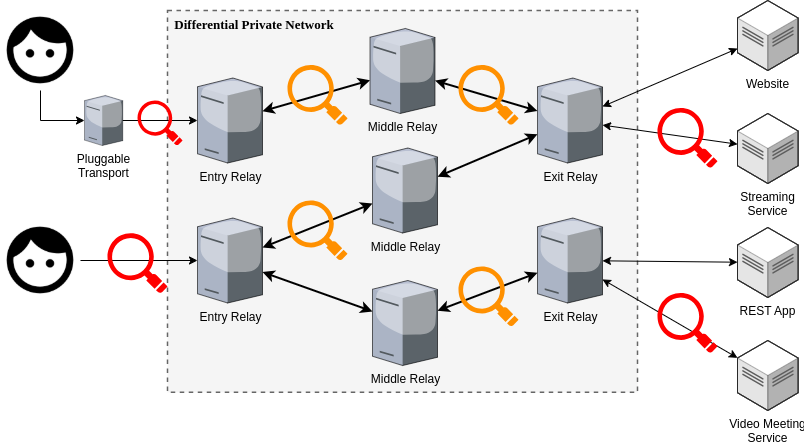
\includegraphics[width=\textwidth]{Chapters/Figures/Threat_Model.png}
  \caption{Threat Model over System Model}\label{fig:thread_model}
\end{figure}

\autoref{fig:thread_model} illustrates the threat model over the system model, showing the adversaries' capabilities and the Tor network segments that they may monitor. The red magnifying glasses indicate the more commonly observed segments of the network, whilst the orange magnifying glasses represent the segments that are less commonly observed. Nonetheless, it is important to note that the adversaries considered by our threat model are not limited to the firstly described segments and our adversaries can monitor any pair of segments in the network.  

For the scope of our solution, we considered SLAd to be the main adversary, as they are more common and realistic in the context of Tor. LSAd are also considered to be a threat and also included in the scope of our threat model, even though we recognize that they are less common. On the other hand, OPAd are not considered in our threat model, as we consider they are not realistic and do not represent a common threat to Tor users.

Building on the original assumptions put forth by~\citeauthor{dingledine2004tor}~\cite{dingledine2004tor}, we consider both passive and active adversaries. A passive adversary merely observes traffic patterns, applying machine learning and data analysis techniques to infer user identities and behaviors, without being able to observe the content of TLS packets. On the other hand, an active adversary compromises onion routers to inject traffic into the network — not merely to observe, but to facilitate more sophisticated traffic analysis attacks. Traffic injection, in this context, becomes a strategic tool for the adversary to train machine learning models capable of uncovering users' identities and tracking their navigation through the Tor network. However, it is important to note that we do not take relay compromise into account. In some context, adversaries may deploy a malicious voluntary relay and our solution might not hold privacy guarantees to users, as the attacker would be able to monitor the traffic patterns and potentially defeat our prototype. 


In summary, our threat model considers powerful State-Level and Large-Scope adversaries capable of monitoring significant portions of the Tor network traffic, but not on its entirety. These adversaries are equipped with advanced and state-of-the-art machine and deep learning and data analysis techniques. These adversaries may be passive, observing traffic patterns, or active by injecting traffic into the network to train their machine learning models. 


\section{Software Architecture}\label{sec:software_architecture}

To ensure a clear understanding of the software architecture of the implemented features Packet Padding Cells and Jitter Induction Schedulers, we will first present the Tor relay architecture, which is the foundation of the presented work, and then we will present the features' architecture, as an extension of the Tor relay architecture.

\subsection{Tor Relay Architecture}\label{sec:tor_relay_architecture}
Tor relays are the backbone of the Tor network, responsible for routing traffic between clients and servers while maintaining user anonymity.  As explained in greater detail in~\autoref{sec:tor_network}, Tor relays are connected through TCP over TLS connections, forming a network of relays that route TLS packets composed by a variable number of cells between clients, relays and servers, encrypting and decrypting the traffic at each hop, layer by layer.

Our solution extends the Tor relay architecture by introducing a pair of new Tor schedulers and a new mechanism for generating additional traffic, presented in~\autoref{sec:system_model}. 
At the time of writing, Tor has 2 types of schedulers: the \textit{KIST} Scheduler, briefly presented in~\autoref{subsubsec:kist}, which also has a \textit{Lite-KIST} variant for low-end devices, and the \textit{Vanilla} Scheduler, which is a simpler scheduler. To develop our solution, we chose to extend both scheduler to provide better insights about the schedulers' performance with our solution, and to allow users to choose the scheduler that best fits their needs.

\begin{figure}[!h]
  \centering
  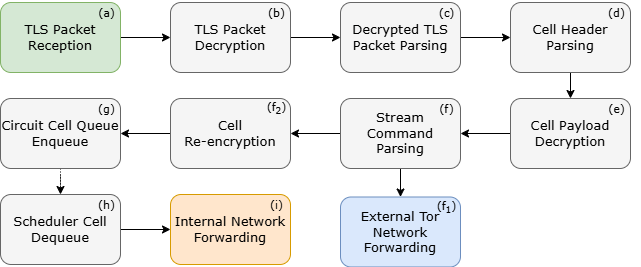
\includegraphics[width=\textwidth]{Chapters/Figures/Tor_Cell_Pipeline.png}
  \caption{Original Cell Processing Pipeline}\label{fig:tor_cell_pipeline}
\end{figure}

To ease the understanding of the Tor relay architecture, we present an  illustration of the pipeline of a Tor cell in a Tor relay in~\autoref{fig:tor_cell_pipeline}. As shown in the figure, after receiving a TLS packet (\(a\)), it gets decrypted (\(b\)) and all Tor cells within the packet are extracted (\(c\)). For each Tor cell within the packet, its header is checked (\(d\))  and its payload gets decrypted (\(e\)). After decrypting the payload, the cell's header \textit{stream command} is used to determine if the relay is the exit and the cell must be forwards to the destination (\(f_1\)), or if the relay corresponds to an entry or middle relay, in which case the cell is forwarded to the next hop. Finally, the cells that must be forwarded are re-encrypted (\(f_2\)) and enqueued in the respective circuit cell queue (\(g\)). The scheduler then dequeues the cells from the circuit cell queue (\(h\)), and forwards them to the next hop (\(i\)).


\subsection{Packet Padding Cells and Jitter Induction Schedulers Architecture}\label{sec:ttt_architecture}

After presenting the Tor relay architecture, together with a better understanding of the Tor cell lifetime in a relay, we can now present the Packet Padding Cells and Jitter Induction Schedulers architecture. As stated in~\autoref{sec:system_model}, our solution brings 2 main features to the Tor project: a new scheduler that applies jitter to the Tor network traffic, and a new mechanism for generation additional traffic.

To allow a better comprehension and comparison to the differences of Tor cells lifetime in the original Tor project and in the proposed solution, we present a similar illustration to~\autoref{fig:tor_cell_pipeline} in~\autoref{fig:ttt_cell_pipeline}, which illustrates the pipeline of a Tor cell in an enhanced relay and identifies the differences introduced by our solution.
\begin{figure}[!h]
  \centering
  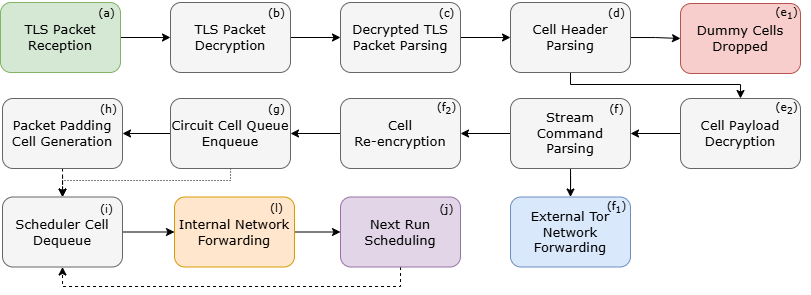
\includegraphics[width=\textwidth]{Chapters/Figures/Solution_Cell_Pipeline.png}
  \caption{PPC and JIS Cell Processing Pipeline}\label{fig:ttt_cell_pipeline}
\end{figure}

Upon receiving a TLS packet (\(a\)), the relay decrypts it (\(b\)) and extracts all cells within the packet (\(c\)), same as the original Tor. For each cell within the packet, the relay checks its header (\(d\)). If the cell is a false cell, it is discarded (\(e_1\)), otherwise the cell is decrypted (\(e_2\)). After decrypting the cell, its \textit{stream command} header is checked to determine if the relay is the exit and the cell must be forwarded to the destination (\(f_1\)), or if the relay corresponds to an entry or middle relay, in which case the cell is forwarded to the next hop. For the cells that must be forwarded, they are re-encrypted (\(f_2\)) and enqueued in the respective circuit cell queue (\(g\)). After queuing a cell, the relay decides, based on a differential private algorithm, if it generates a new false cell (\(h\)). Newly generated cells are added to the circuit cell queue of the original cell. Once any cell is added to the circuit cell queue, the circuit is marked to inform other components that it is ready to sent cells outwards, leading the scheduler to dequeue the cells from the circuit cell queue (\(i\)). After being dequeued, cells are placed in the output buffer for retransmission, and forwarded the cells to the next hop (\(l\)). Meanwhile, the scheduler calculates if jitter must be applied to the circuit, therefore setting a random interval between the time of the last scheduler run and the next, based on a configurable and pre-determined mathematical distribution and randomness parameters (\(j\)), impacting the following cells time of retransmission. 

In comparison to the original Tor cell pipeline, the main differences are the step (\(e_1\)), where the false cells are discarded, the step (\(i\)), where the process of decision and generation of \textit{Packet Padding Cells} takes place, and the step (\(m\)), where the scheduler randomly decides when the next run will be. The Schedulers implement jitter into the Tor network by calculating the next time the scheduler will run again based on a random delay, which is calculated based on the differential private algorithm, and executing this calculation after performing the circuit queues operations to avoid performance issues with such operations.
\begin{figure}[!h]
  \centering
  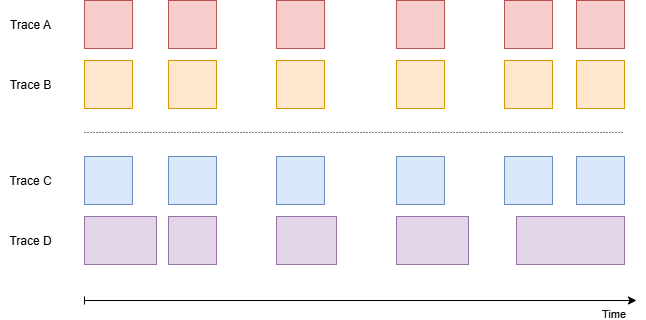
\includegraphics[width=\textwidth]{Chapters/Figures/PPC_Timeline.png}
  \caption{Packet Padding Cells Feature Timeline Overview}\label{fig:ppc_timeline}
\end{figure}

\begin{figure}[!h]
  \centering
  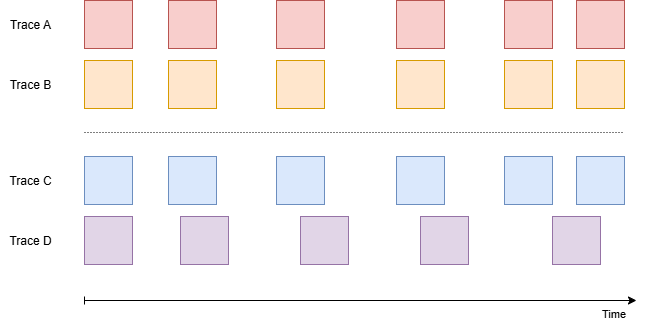
\includegraphics[width=\textwidth]{Chapters/Figures/JIS_Timeline.png}
  \caption{Jitter Induction Schedulers Feature Timeline Overview}\label{fig:jis_timeline}
\end{figure}

Even though we present these features together, it is important to note that they are independent, can be used separately, and focus on different aspects of the Tor network to produce unobservability and enhance its resistance against traffic analysis attacks. 

In~\autoref{fig:ppc_timeline} and~\autoref{fig:jis_timeline}, we present a timeline overview of both features, illustrating examples of TLS packets traces over a given time window and how the features impact the Tor network traffic. In this example, consider that an attacker is monitoring the traffic between the client and the first relay, corresponding to traces A and C in the figures, and between the last relay and the destination server, corresponding to trace B and D in the figures, and that the adversary captures the traffic in a certain time window. The top example of both figures illustrates the original Tor traffic, without any of our features, where the traffic pattern is clearly observable in both traces of the network. This way, an attacker can analyze the traffic patterns and potentially de-anonymize users and expose their browsing activities. On the bottom of both figures, we illustrate the traffic patterns when our features are applied to the Tor network, individually. 

In the case of Packet Padding Cells, the generated false cells create noise in the traffic patterns, more specifically in the size of the TLS packets, making the traffic patterns less observable and more difficult to analyze. Additionally, if we consider an additional segment of the network, the 3 traces would also appear different, as the false cells are generated independently in each relay and are discarded on reception.

In the case of Jitter Induction Schedulers, the jitter applied by the developed schedulers creates variability in the timing of the TLS packets, once again working as noise in the traffic patterns and improving the Tor network's resistance against traffic analysis attacks. These illustrations highlight the aspects in which each feature impacts the Tor network traffic, and how they can be used together to provide a more robust defense against traffic analysis attacks. This feature also impacts the network performance over time, as the delays added by the Schedulers accumulate over time and propagate through each hop.

The Packet Padding Cells mechanism focuses on obfuscating traffic patterns by randomizing the TLS Packet size through false cells' generation, while the Jitter Induction Schedulers aim to introduce variability in the timing of TLS packets, making it more challenging for adversaries to analyze traffic patterns.

\section{Parameterization}\label{sec:parameterization}

Our solution extends Tor with 2 new features to enhance its resistance against traffic analysis attacks, and we aim to provide users and hosts with full control over the privacy and performance trade-offs. To do so, the parameterization of our solution must be user-friendly and easy to configure, without requesting users to have a deep understanding of the underlying mechanisms 


\subsection{Used Techniques}\label{sec:used_techniques}

The Tor project handles its configuration through a key-value file called \texttt{torrc}. This file is used as a single point of configuration for the Tor network, allowing users and hosts to define the type of relay, to set various parameters such as bandwidth limits and to configure the behavior of the Tor software. Some configuration parameters also allow the software to swap configuration mid-execution, without the need to restart the Tor process.

Our solution extended the existing Tor configuration file to include new parameters that allow users and hosts to configure the behavior of the new Schedulers and the Packet Padding Cells mechanism. These parameters are designed to give full control to users and hosts, allowing them to choose the level of privacy they want to achieve.


\subsection{Jitter Parameterization}\label{sec:jitter_parameterization}

To configure the Tor software to use our Schedulers and configure the injection of jitter into the network traffic, we extended the torrc file with the following parameters: 

\paragraph{Schedulers} As mentioned before, this parameter was already present in the Tor project, and was extended to accept the new Schedulers, \texttt{PRIV\_KIST} and \texttt{PRIV\_Vanilla}. 

\paragraph{PrivSchedulerEpsilon} Similar to the \texttt{DummyCellEpsilon} parameter, this parameter is used to define the variability of the jitter applied by the Schedulers. As an inspired Differential Privacy parameter, the value must be greater or equal than 0, and the higher the value, the less jitter will be applied, therefore the less privacy will be provided. The default value is set to -1, which turns the jitter off. When the jitter is turned off, the scheduler will behave as its original version.  

\paragraph{PrivSchedulerDistribution} This parameter is used to define the distribution used to generate the time intervals between scheduler runs. At the moment, the Schedulers only accept the following distributions: \textit{Uniform}, \textit{Laplace}, \textit{Poisson}, \textit{Exponential} and \textit{Normal}. By default, if one of our Schedulers is used and no distribution is set, the Tor software will exit with an error.

\paragraph{PrivSchedulerMinJitter} This parameter sets the minimum possible interval between two consecutive scheduler runs. The default value is set to 1.

\paragraph{PrivSchedulerMaxJitter} Similarly to the \texttt{PrivSchedulerMinJitter} parameter, this parameter sets the maximum possible interval between two consecutive scheduler runs. The default value is set to 10. 

\paragraph{PrivSchedulerTargetJitter} To give more control to the user, this parameter is used to set the target jitter that the Schedulers should aim to achieve. The Schedulers will try to apply a random delay between the minimum and maximum jitter, with center in this parameter. The default value is set to 2.\linebreak

These last 3 parameters are tightly related and the Tor software will exit with an error if \texttt{PrivSchedulerMinJitter} $\le$ \texttt{PrivSchedulerTargetJitter} $\le$ \texttt{PrivSchedulerMaxJitter}.

These parameters allow users to configure the jitter generation process, by defining a randomness Differential Privacy-inspired variable and an interval of possible outcomes. We also integrated some of the most common mathematical distributions to generate the random numbers, allowing users to choose the distribution that best fits their needs and to allow the jitter conditions among several network segments to behave differently.  
\subsection{Packet Padding Cells Parameterization}\label{sec:packet_padding_parameterization}

The \textit{Packet Padding Cells} feature is a simple mechanism that generates additional traffic with a Differential Private Randomized Response mechanism. To keep this feature as simple and user-friendly as possible, we extended the torrc file with the following parameter:

\paragraph{DummyCellEpsilon} This is the only configuration parameter used for the Packet Padding Cells mechanism. It is used to set the Differential Privacy parameter $\epsilon$ value for the decision-making algorithm that generates the Packet Padding Cells. By default, the value is set to -1, which turns the mechanism off. As a Differential Privacy parameter, the value must be greater than 0, and the higher the value, the fewer cells will be generated, therefore the less privacy will be provided. The highest possible ratio of generated cells in relation to the original cells is 0.5, when this parameter is set to 0.

With just one parameter, users and host are able to configure the Packet Padding Cells mechanism, allowing them to choose the level of privacy they want to achieve. 


\section{Summary}\label{sec:architeture_discussion}

In this chapter, we presented an in-depth analysis of the system model and software architecture of the proposed Packet Padding Cells and Jitter Induction Schedulers features. We began by introducing the overall objectives and foundational principles of the system, and discussed the goals of the proposed solution and how they align with the principles of the Tor project, ensuring compatibility and unobservability while maintaining performance. The threat model was analyzed, focusing on potential adversaries and their capabilities, particularly in relation to traffic analysis attacks and with state of the art. Then, we delved into the software architecture, illustrating the Tor relay architecture and how our features extend it, explaining the lifecycle of a Tor cell within a relay and the modifications introduced by our solution, and they impact on the Tor network traffic. Finally, we presented the parameterization of both features, emphasizing user-friendliness and configurability to allow users and hosts to tailor the privacy-performance trade-offs according to their needs.

